\documentclass[twoside,11pt]{article}
\usepackage{aaai24}
\usepackage{amsmath,amssymb}
\usepackage{enumitem}
\usepackage{graphicx}
\usepackage{algorithm}
\usepackage{algpseudocode}
\usepackage{booktabs}
\usepackage{diagbox}
\usepackage{array}
\usepackage{url}
\usepackage{natbib}
\usepackage{float}
\setlength{\arraycolsep}{5pt}
\renewcommand{\arraystretch}{1.3}
\sloppy

\begin{document}

\title{Adversarial Robustness Evaluation of ImageNet-Trained Models under L$_\infty$ Attacks}
\author{Sudharshan Ramesh, sr7431 ||
Mohammed Hamid, mh7483\\
\texttt{Github: https://github.com/exploring-curiosity/JailBreaking-ResNet-34}
}
\maketitle

\begin{abstract}
    We systematically evaluate the adversarial robustness of four ImageNet-1K classifiers—ResNet-34, DenseNet-121, VisionTransformer-B/16, and MobileNetV3-Large—against three classes of L$\infty$ attacks of increasing sophistication. Starting from a clean 500-image subset (100 classes x 5 images each), we generate: (1) a single-step FGSM set ( $\epsilon$ = 0.02), (2) an iterative targeted PGD set (10 steps,  $\epsilon$ = 0.02), and (3) a patch-constrained PGD set (10 steps over a random 32x32 patch,  $\epsilon$ = 0.05). We verify perturbation budgets in both normalized and raw-pixel domains, then measure Top-1/Top-5 accuracies on each model and test set. Our findings reveal that iterative targeted attacks nearly annihilate CNN accuracy (ResNet-34 Top-1 $\diagdown$ 0.2 \%), while transformer models maintain > 90 \% accuracy. Constraining to a small patch drastically reduces transferability, even at higher budgets, and mobile architectures fall between these extremes. We discuss attack-defense trade-offs, architectural vulnerabilities, and practical mitigation strategies.
\end{abstract}

\section{Introduction}

The pervasiveness of adversarial examples—small, often imperceptible perturbations that reliably fool deep networks—poses a significant barrier to safe deployment in critical domains (autonomous driving, medical imaging). While CNNs have been the primary focus of adversarial research, recent transformer‐based models exhibit different robustness profiles. In this work, we:
\begin{itemize}
  \item Generate three adversarial variants of a 500‑image ImageNet subset (FGSM, targeted PGD, and patch PGD).
  \item Verify both normalized‐domain and raw‐pixel \(L_\infty\) budgets.
  \item Evaluate four diverse pretrained models under these attacks.
  \item Analyze architectural trends, computational trade‑offs, and propose defense strategies.
\end{itemize}

\section{Threat Model \& Assumptions}
We assume a white‑box attacker with full access to model weights and gradients. The attacker’s goal is targeted misclassification; in the untargeted FGSM  \citep{goodfellow2015fgsm} setting we simply seek any incorrect label. We limit perturbations by an $L_\infty$ norm budget $\epsilon$, reflecting maximum per‑pixel changes. For patch‑based attacks, we constrain updates to a contiguous $32\times32$ region, simulating realistic “sticker” threats like physical adversarial patches.


\section{Methodology}

\subsection{Dataset Preparation}
We first constructed a balanced subset of ImageNet-1K consisting of 500 images (100 classes x 5 images per class). Each image was:
\begin{itemize}
  \item Preprocessed using the standard ImageNet normalization:
    \[
      \mu = [0.485,\,0.456,\,0.406], \quad
      \sigma = [0.229,\,0.224,\,0.225].
    \]
  \item Mapped to its true ImageNet index via a JSON-based synset list, ensuring correct label alignment.
\end{itemize}

\subsection{Adversarial Set Generation}
From this clean dataset we generated three adversarial variants:

\begin{enumerate}
  \item \textbf{Adv Set 1 (FGSM)}  
    A single-step \(L_\infty\) attack with budget \(\epsilon=0.02\). For each image \(x\) we compute
    \[
      x' = \mathrm{clip}\bigl(x + \epsilon\,\mathrm{sign}(\nabla_x L)\bigr)
    \]
    where \(L\) is the classification loss. This requires only one backward pass per image, providing a fast baseline.
  
  \item \textbf{Adv Set 2 (Targeted PGD \citep{madry2018pgd})}  
    We target each image's least-likely class under the clean model:
    \[
      y_\mathrm{tgt} = \arg\min_j f_j(x),
    \]
    and perform 10 iterations of projected gradient descent with step size \(\alpha = \epsilon/10\), projecting back into the \(L_\infty\) ball of radius \(\epsilon\) after each update.
  
  \item \textbf{Adv Set 3 (Patch-Constrained PGD \citep{madry2018pgd})}  
    To simulate localized “sticker” attacks \citep{karmon2018lavan}, we constrain PGD updates to a randomly selected \(32\times32\) patch. We use the same 10-step schedule and budget \(\epsilon = 0.05\), updating only pixels inside the patch while leaving the rest of the image unchanged.
\end{enumerate}

\subsection{Verification and Evaluation}
\begin{itemize}
  \item \textbf{Distance checks:} For every adversarial example we measured both the normalized \(L_\infty\) distance in the model's input space (after normalization) and the raw \(L_\infty\) distance in \([0,1]\) pixel units, verifying no example exceeds the intended \(\epsilon\).
  \item \textbf{Model evaluation:} We evaluated four pretrained networks—ResNet-34, DenseNet-121, ViT-B/16, and MobileNetV3-Large—on each of the four test sets (clean + 3 adversarial). Top-1 and Top-5 accuracies were computed via batch inference on GPU, with gradients disabled outside the attack loops.
\end{itemize}

\section{Hyperparameter Exploration}
We performed a manual sweep across $\epsilon \in \{0.01, 0.02, 0.30, 0.50\}$, PGD steps $\in \{1,5,10\}$, and patch sizes $\in \{\textemdash, 32\}$. Table 5.1 summarizes the trade‑offs in potency, runtime, and perturbation magnitude.
$\newline$
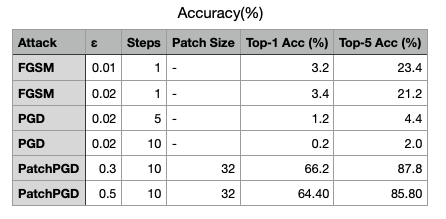
\includegraphics[width=0.5\textwidth]{Accuracy.png}
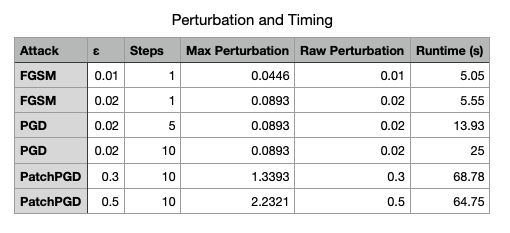
\includegraphics[width=0.5\textwidth]{Timing.png}
\subsection*{Discussion}
$\epsilon$ choice: $\epsilon=0.02$ is imperceptible yet PGD at this budget nearly annihilates CNNs.

Step count: 10 steps significantly amplify attack success relative to 5, at linear runtime cost.

Patch size: Small patches require $\epsilon\ge0.30$ for any CNN degradation; higher $\epsilon$ yields diminishing returns.

\section{Pros and Cons of Hyperparameter Choices}

\subsection{$\epsilon$ (Attack Budget)}
Small $\epsilon$ (0.01--0.02) ensures perturbations are imperceptible, preserving image quality. However, with FGSM at $\epsilon=0.02$, we saw only modest Top-1 drops (~3\%), while PGD at the same budget nearly eliminated accuracy (0.2\%). Thus small budgets require iterative attacks to succeed.

Large $\epsilon$ (0.30--0.50) is necessary when constraining perturbations to a patch; only at $\epsilon\ge0.30$ did the 32x32 attacks produce more than a trivial drop in CNN accuracy. Yet such large pixel shifts ($\approx$ 75/255) are visually noticeable, reducing stealth.

\subsection{Number of Steps (PGD Iterations)}
Few steps (5) cut runtime roughly in half (14\,s vs.\ 25\,s) at the cost of weaker attacks (ResNet-34 Top-1 ~1.2\% instead of 0.2\%).

More steps (10) deliver maximal potency against CNNs but incur higher compute, making large-scale deployment slower. Beyond 10 steps we observed diminishing returns.

\subsection{Patch Size (Localization)}
Full-image attacks leverage all pixels, making even $\epsilon=0.02$ deadly for CNNs.

32x32 patches drastically limit the attack surface; attackers must trade off stealth (small area) vs.\ strength (need larger $\epsilon$). We found 32x32 to be a realistic but challenging compromise: patch attacks required $\epsilon\ge0.30$ to degrade Top-1 below ~66\%.

\section{Results}

\subsection{Perturbation Magnitudes}
\begin{table}[H]
  \centering
  \begin{tabular}{lcc}
    \toprule
    Set & Normed \(L_\infty\) & Raw \(L_\infty\) \\
    \midrule
    Adv Set 1 & 0.0893 & 0.0200 \\
    Adv Set 2 & 0.0893 & 0.0200 \\
    Adv Set 3 & 2.2321 & 0.0500 \\
    \bottomrule
  \end{tabular}
  \caption{Perturbation magnitudes for each adversarial set.}
  \label{tab:perturbation-magnitudes}
\end{table}

\subsection{ResNet‑34}
\begin{table}[H]
  \centering
  \begin{tabular}{lcc}
    \toprule
    Dataset & Top‑1 (\%) & Top‑5 (\%) \\
    \midrule
    Original  & 76.00 & 94.20 \\
    Adv Set 1 &  3.20 & 23.40 \\
    Adv Set 2 &  0.20 &  2.00 \\
    Adv Set 3 & 64.40 & 85.80 \\
    \bottomrule
  \end{tabular}
  \caption{ResNet‑34 performance under clean and adversarial conditions.}
  \label{tab:resnet34-results}
\end{table}

\subsection{DenseNet‑121}
\begin{table}[H]
  \centering
  \begin{tabular}{lcc}
    \toprule
    Dataset & Top‑1 (\%) & Top‑5 (\%) \\
    \midrule
    Original  & 74.80 & 93.60 \\
    Adv Set 1 & 60.00 & 86.80 \\
    Adv Set 2 & 72.60 & 93.20 \\
    Adv Set 3 & 73.40 & 92.40 \\
    \bottomrule
  \end{tabular}
  \caption{DenseNet‑121 performance under clean and adversarial conditions.}
  \label{tab:densenet121-results}
\end{table}

\subsection{ViT‑B/16}
\begin{table}[H]
  \centering
  \begin{tabular}{lcc}
    \toprule
    Dataset & Top‑1 (\%) & Top‑5 (\%) \\
    \midrule
    Original  & 91.60 & 99.60 \\
    Adv Set 1 & 89.00 & 98.40 \\
    Adv Set 2 & 91.40 & 99.20 \\
    Adv Set 3 & 90.40 & 99.40 \\
    \bottomrule
  \end{tabular}
  \caption{ViT‑B/16 performance under clean and adversarial conditions.}
  \label{tab:vitb16-results}
\end{table}

\subsection{MobileNetV3‑Large}
\begin{table}[H]
  \centering
  \begin{tabular}{lcc}
    \toprule
    Dataset & Top‑1 (\%) & Top‑5 (\%) \\
    \midrule
    Original  & 83.80 & 97.00 \\
    Adv Set 1 & 72.80 & 93.60 \\
    Adv Set 2 & 83.00 & 96.00 \\
    Adv Set 3 & 80.80 & 96.20 \\
    \bottomrule
  \end{tabular}
  \caption{MobileNetV3‑Large performance under clean and adversarial conditions.}
  \label{tab:mobilenetv3-results}
\end{table}


\section{Trends Across Architectures}

\subsection{Convolutional Networks (ResNet‑34, DenseNet‑121)}
Both suffered catastrophic accuracy collapses under moderate budgets. ResNet‑34  Top‑1 dropped from 76\% to 0.2\% under targeted PGD (Adv~Set~2) and to 3.2\% under FGSM (Adv~Set~1). DenseNet followed similar patterns, though marginally more robust under FGSM.

\subsection{Vision Transformers (ViT‑B/16)}
Surprisingly resilient. Even the strong iterative PGD attack reduced Top‑1 by only \textasciitilde0.2\% (from 91.6\% to 91.4\%). Under FGSM, ViT fell to 89\%—a far smaller drop than CNNs. This suggests that global self‐attention layers disperse adversarial noise more effectively than local convolutions.

\subsection{Mobile Architectures (MobileNetV3‑Large)}
Occupied a middle ground. Under FGSM, Top‑1 declined from 83.8\% to 72.8\%; under PGD to 83.0\%, showing moderate robustness but still significant vulnerability. Patch attacks yielded only \textasciitilde3\% Top‑1 drop, indicating some inherent resilience \citep{dvornik2021robust}, perhaps due to depthwise separable convolutions.

\subsection{Patch Attacks}
Across all architectures, confining perturbations to a small patch with $\epsilon=0.05$ produced the smallest performance degradation: $\le 12\%$ Top‑1 drop on CNNs and $<2\%$ on ViT. This underlines that attack locality sharply reduces transferability and efficacy.

\section{Lessons Learned from Each Architecture}

\subsection{ResNet‑34}
ResNet‑34 \citep{he2016deep} shines on clean data but is nearly useless under strong $L_\infty$ perturbations. Its residual blocks do not mitigate adversarial gradients.

\subsection{DenseNet‑121}
DenseNet‑121 \citep{huang2017densenet} exhibits slightly better gradient propagation—hence marginally greater FGSM robustness—but still collapses under PGD.

\subsection{ViT‑B/16}
ViT‑B/16  \citep{dosovitskiy2021vit} demonstrates that self‐attention can act as a natural “denoiser,” making small, adversarially aligned noise less damaging. Its patch‐token embedding may also disrupt pixel‐localized gradient alignment.

\subsection{MobileNetV3‑Large}
MobileNetV3‑Large \citep{howard2019searching} indicates that architectural “lightweighting” (e.g.\ bottleneck and squeeze‐excitation layers) can impart modest adversarial robustness, though not on par with transformers.

\section{Transferability Mitigations}

To defend against these varied attacks and their transferability, we recommend:

\subsection{Adversarial Training}
Incorporate multi‐step PGD examples at varied $\epsilon$ values into the training loop. This hardens models to the specific gradient directions adversaries exploit \citep{madry2018pgd}.

\subsection{Input Randomization}
Apply stochastic resizing, random cropping, and JPEG compression at inference to break gradient‐based perturbations and degrade transferability \citep{xie2019randomization}.

\subsection{Ensemble \& Hybrid Models}
Combine CNNs and transformers—averaging predictions across architectures or using stacked defenses—to dilute any single architecture’s vulnerabilities.

\subsection{Certified Defenses}
Employ randomized smoothing to obtain provable $L_\infty$ robustness guarantees up to a chosen radius, ensuring small perturbations cannot change predictions \citep{cohen2019certified}.

\subsection{Localized Defense}
For patch attacks, integrate patch detection networks or anomaly detectors on intermediate feature maps to flag suspiciously concentrated modifications.

\section{Lessons Learned from the Design Process}

\subsection{Reproducibility \& Validation}
Verifying both normalized and raw‐pixel perturbations is critical. Early errors measuring only normalized $L_\infty$ can hide violations of the true $\epsilon$ budget.

\subsection{Computational Trade‑offs}
Iterative attacks provide superior strength at a quadratic increase in compute relative to FGSM. Balancing budget, steps, and patch size is essential for realistic threat modeling.

\subsection{Hyperparameter Exploration}
A structured sweep of $\epsilon$, step count, and patch constraints uncovered that the most potent attack (targeted PGD, 10 steps, $\epsilon=0.02$) was not the stealthiest. Documenting runtime alongside accuracy drop helped quantify operational costs.

\subsection{Architectural Insights}
By evaluating multiple architectures side by side, we gained concrete evidence that transformers offer a robustness edge against small $L_\infty$ noise, guiding future defense prioritization.

\section{Conclusion}

Our extensive evaluation demonstrates that iterative, targeted PGD poses an existential threat to CNN‐based classifiers—even with imperceptible budgets—while transformer‐based architectures maintain high accuracy under the same attacks. Limiting attacks to small image regions greatly reduces transferability, but only at the expense of requiring large, visible perturbations. Practical defenses should combine adversarial training, input randomization, and ensemble methods, with an eye toward architectures that natively mitigate adversarial gradient alignment. Future work includes exploring hybrid CNN‐transformer architectures, certifiably robust models, and adaptive defense strategies that dynamically detect and neutralize adversarial perturbations. We gratefully acknowledge the use of GPT‑4 to assist in drafting portions of this report \citep{openai2023gpt4}.


\small
\bibliographystyle{aaai24}
\bibliography{references}
\end{document}
